% Тут используется класс, установленный на сервере Papeeria. На случай, если
% текст понадобится редактировать где-то в другом месте, рядом лежит файл matmex-diploma-custom.cls
% который в момент своего создания был идентичен классу, установленному на сервере.
% Для того, чтобы им воспользоваться, замените matmex-diploma на matmex-diploma-custom
% Если вы работаете исключительно в Papeeria то мы настоятельно рекомендуем пользоваться
% классом matmex-diploma, поскольку он будет автоматически обновляться по мере внесения корректив
%

% По умолчанию используется шрифт 14 размера. Если нужен 12-й шрифт, уберите опцию [14pt]
%\documentclass[14pt]{matmex-diploma}
\documentclass[14pt]{matmex-diploma-custom}

\hyphenation{op-tical net-works semi-conduc-tor con-tract Et-he-re-um}
\hyphenation{пре-по-да-ва-тель сту-дент вы-чис-ли-тель-но}
\newcommand\name[1]{\textsc{#1}}
\newcommand\achtung[1]{{\color{red}#1}}

\usepackage{graphicx}
\usepackage{listings}


\begin{document}
% Год, город, название университета и факультета предопределены,
% но можно и поменять.
% Если англоязычная титульная страница не нужна, то ее можно просто удалить.
\filltitle{ru}{
    chair              = {Программная инженерия\\ Кафедра системного программирования},
    title              = {Специализация алгоритма Витерби на GPGPU скрытой марковской моделью},
    % Здесь указывается тип работы. Возможные значения:
    %   coursework - Курсовая работа
    %   diploma - Диплом специалиста
    %   master - Диплом магистра
    %   bachelor - Диплом бакалавра
    type               = {master},
    author             = {Тюляндин Иван Владимирович},
    supervisorPosition = {к.\,ф.-м.\,н., доцент},
    supervisor         = {С.\,В. Григорьев},
    consultantPosition   = {программист ООО "Интеллиджей Лабс"\\ к.\,ф.-м.\,н.},
    consultant           = {Д.\,А. Березун},
    reviewerPosition   = {},
    reviewer           = {}
%   university         = {Санкт-Петербургский Государственный Университет},
%   faculty            = {Математико-механический факультет},
%   city               = {Санкт-Петербург},
%   year               = {2013}
}
\filltitle{en}{
    chair              = {Software Engineering},
    title              = {Specialization of GPGPU implemented Viterbi algorithm with hidden Markov model},
    author             = {Ivan Tyulyandin},
    supervisorPosition = {Assistant Professor, PhD},
    supervisor         = {Semyon Grigorev},
    consultantPosition   = {IntelliJ Labs Co. Ltd developer\\ PhD},
    consultant           = {Daniil Berezun},
    reviewerPosition   = {},
    reviewer           = {}
    % chairHeadPosition  = {professor},
    % chairHead          = {Christobal Junta},
}
\maketitle
\tableofcontents
% У введения нет номера главы

\section*{Введение}

Скрытые марковские модели~\cite{HMM_wiki}.

\section{Постановка задачи}
Цель данной работы --- исследовать применимость специализации алгоритма Витерби, реализованного на GPGPU.

Были поставлены следующие задачи:
\begin{itemize}
	\item сделать обзор предметной области и существующих решений задачи 
		гомологичности;
	\item написать специализатор алгоритма Витерби на СММ;
	\item провести сравнительный анализ специализированной программы с
		существующими решениями.
\end{itemize}

\section{Обзор}
В разделе рассмотрены терминология и технологии программирования гетерогенных
вычислительных систем, в которых центральный процессор (CPU) управляет GPGPU, 
скрытые марковские модели и их применение в задаче гомологичности.
Сделан обзор существующего программного обеспечения, решающего задачу
гомологичности.

\subsection{Терминология гетерогенных систем}
Программирование гетерогенных систем использует модель вычислений \name{SPMD} 
(Single Program Multiple Data).
В этой модели одна программа выполняется параллельно на
различных физических устройствах, каждое из которых обрабатывает часть данных и
имеет свой программный счетчик.
Наличие счетчика является главным отличием от модели \name{SIMD} (Single
Instruction Multiple Data), где одновременно на всех устройствах выполняется
одна и та же инструкция.
Более подробное определение терминов \name{SPMD}, описанных ниже, можно 
посмотреть в спецификации стандарта \name{OpenCL}~\cite{OpenCL_spec}.

\emph{Устройство} --- составная часть гетерогенной вычислительной системы.
Устройством может быть CPU или GPGPU.

\emph{Ядро} --- код, предназначенный для параллельного выполнения на
устройстве.
	
\emph{Поток исполнения} --- логический вычислитель, выполняющий ядро.
Поток можно идентифицировать внутри ядра по уникальному номеру.

\emph{Рабочая группа} --- это фиксированное множество потоков исполнения,
которые выполняют одно ядро и имеют общий участок памяти.
Потоки внутри группы могут быть синхронизированы с помощью барьера.
Рабочая группа также имеет уникальный номер.

\emph{Приватная память} --- область памяти потока исполнения. 
К переменным, объявленным в этой памяти, другие потоки исполнения не могут 
обратиться.

\emph{Локальная память} --- область памяти рабочей группы, которая доступна
всем потокам исполнения этой группы для взаимодействия.

\emph{Глобальная память} --- память, которую любой поток исполнения может считывать и перезаписывать.

\emph{Неизменяемая память} -- участок глобальной памяти, данные в котором не меняются во время выполнения ядра.

Различные виды памяти имеют разную скорость доступа к данным.
Наибольшая задержка доступа у глобальной памяти, которая является отдельным модулем устройства.
Неизменяемая память, как правило, чуть быстрее, так как не нужно задействовать
механизмы когерентности данных.
Некоторые участки глобальной памяти могут быть помещены в кэш устройства, что ускорит последующие обращения к ним.
Локальная память располагается ближе к физическим вычислителям соответствующей 
рабочей группы, поэтому она производительнее по сравнению с глобальной и 
неизменяемой памятью.
Приватная память самая эффективная по скорости доступа к данным.
Эта память является регистрами физического вычислителя, на котором запущен 
поток исполнения.

\subsection[Технологии программирования гетерогенных систем] {Технологии
программирования гетерогенных\\ систем}
Здесь кратко описаны различные языки программирования систем вида 
CPU и GPGPU, а также их инфраструктура.

\subsubsection{\name{NVIDIA CUDA}}
\name{CUDA} (Compute Unified Device Architecture)~\cite{CUDA} --- 
это платформа параллельных вычислений и программный интерфейс 
для управления видеокартами.
\name{CUDA} является пропиетарной разработкой компании \name{NVIDIA}.
Исходный код на \name{CUDA} транслируется в \name{PTX} ---
псевдо-ассемблерное промежуточное представление, 
которое драйвер видеокарты переводит в бинарный код.
\name{CUDA} предназначена только для работы с GPGPU от \name{NVIDIA}.

\subsubsection{\name{OpenCL} и \name{SYCL}}
Разнообразие оборудования и интерфейсов усложняет поддержку
программного обеспечения.
Представителями индустрии была сформирована \name{Khronos Group} с целью
разработки общих открытых стандартов программирования гетерогенных
вычислительных систем.

Одним из результатов работы группы стал стандарт 
\name{OpenCL}~\cite{OpenCL} --- программный интерфейс для использования любого
устройства, которое предоставляет соответствующий драйвер.
Для разработки кода ядра используется диалект
языка \name{C99} с некоторыми ограничениями.
В \name{OpenCL} программист должен явно указывать, каким образом и когда
передавать данные на требуемое устройство.
Изначально ядро нужно было компилировать во время исполнения, 
то есть каждый раз при запуске программы, даже если само ядро не менялось.
Такой вариант называется онлайн компиляцией, которая необходима для 
обеспечения переносимости.

Позднее появился стандарт \name{SPIR-V}~\cite{SPIR-V}, описывающий
переносимое промежуточное представление.
\name{SPIR-V} можно транслировать в \name{LLVM IR}~\cite{LLVM} и наоборот.
Стало возможным единовременно компилировать весь исходный код с помощью 
инфраструктуры \name{LLVM}.
Способ, когда ядро во время сборки приложения компилируется в
\name{SPIR-V}, а затем используется \name{LLVM}, 
называется оффлайн компиляцией.

Наличие этих двух стандартов привело к созданию \name{SYCL}~\cite{SYCL}.
Это высокоуровневая абстракция на \name{С++} над \name{OpenCL} с полной
обратной совместимостью.
В отличие от \name{OpenCL}, в \name{SYCL} управление памятью автоматическое.
Программист должен указать, какие данные требуются для выполнения ядра на
конкретном устройстве.
Затем на стадии компиляции строится граф зависимости данных между 
ядрами, на основе которого генерируется код управления памятью.
Ядро пишется на стандартном \name{C++} с некоторыми ограничениями --- 
нельзя использовать исключения, указатели на функции и виртуальные функции, 
но можно применять лямбда-выражения, шаблоны, наследование и другие абстракции.
Такой дизайн (рис.~\ref{SYCL_infrastructure}) позволяет компилятору 
использовать инфраструктуру компилятора \name{C++} для создания
оптимизированного кода.
\begin{figure}
  \centering
  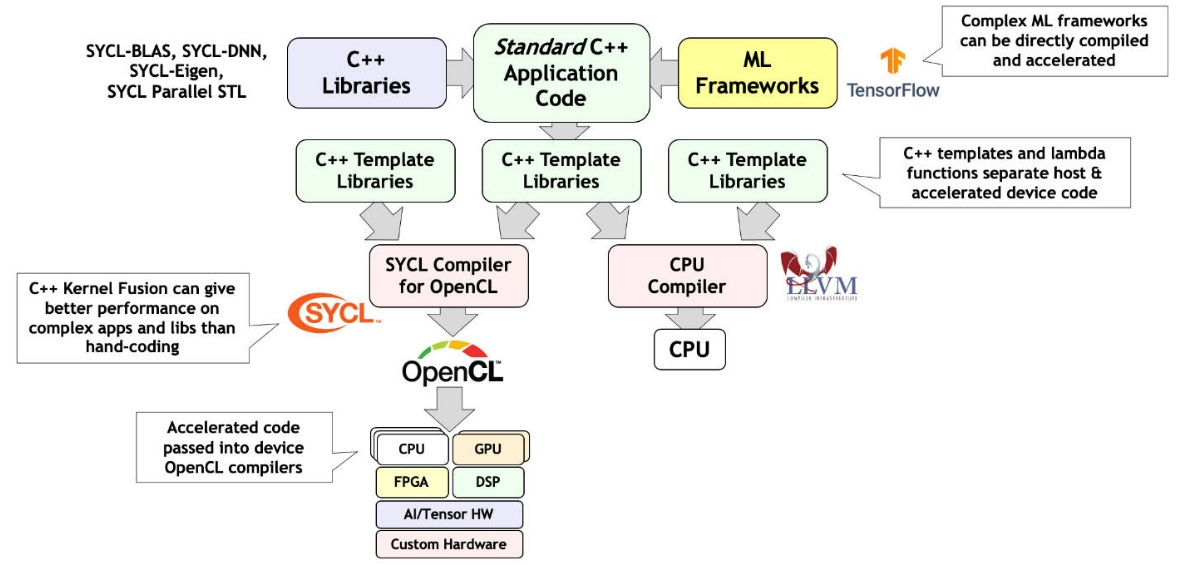
\includegraphics[width=\columnwidth]{sycl.jpg}
  \caption{Инфраструктура приложения с использованием \name{SYCL}~\cite{SYCL}}
  \label{SYCL_infrastructure}
\end{figure}

Сейчас есть четыре реализации стандарта \name{SYCL}: 
\name{ComputeCpp}~\cite{ComputeCpp} от Codeplay,
\name{DPC++}~\cite{DPC} от \name{Intel},
\name{hipSYCL}~\cite{hipSYCL},
\name{triSYCL}~\cite{triSYCL} от \name{AMD} и \name{Xilinx}.
Первая реализация распространяется бесплатно в виде разделяемой библиотеки,
остальные являются проектами с открытым исходным кодом.
На данный момент \name{ComputeCpp} является наиболее соответствующей 
стандарту реализацией.
Также идет работа над тем, чтобы транслировать код с использованием \name{SYCL} 
на эквивалентный \name{CUDA} код, так как приложения на \name{OpenCL} или
\name{SYCL} для GPGPU от \name{NVIDIA} менее производительны, чем аналогичные 
на \name{CUDA} из-за ограниченной поддержки стандарта \name{OpenCL} на этих 
устройствах со стороны \name{NVIDIA}.

\subsection{СММ и алгоритм Витерби}
Скрытая марковская модель~(СММ) является дискретным вероятностным автоматом.
Модель имеет следующие параметры: множество состояний $St_{1..k}$, множество 
наблюдаемых событий $Obs_{1..n}$, вероятности $Pr\_b_{1..k}$ состояний быть
начальными, матрица $Tr$ вероятностей переходов между состояниями размера $k
\times k$ и матрица $Em$ вероятностей наблюдения события в определённом 
состоянии размера ${k\times n}$.

Алгоритм Витерби (лист.~\ref{Viterbi}) используя технику динамического 
программирования считает по наблюдениям $O$ в моменты времени от 1 до
$t$ вероятность оказаться в состоянии $S$ в момент времени $t$.

\begin{lstlisting}[caption=Псевдокод алгоритма Витерби, label=Viterbi, escapeinside={(*}{*)}]
function Viterbi(St, Obs, Pr_b, Tr, Em, O, S)
	Dp[1..t][1..k]

	for j = 1..k
		Dp[1][j] = Pr_b[j] * Em[j][O[1]]
	
	for i = 2..t
		for j = 1..k
			Dp[i][j] = (*$\max_{x = 1..k}$*)(Dp[i - 1][x] * Tr[x][j] * Em[j][O[i]])

	return Dp[t][S]
\end{lstlisting}

\subsection{Задача гомологичности}
В этом подразделе рассмотрена задача гомологичности и способ её решения с 
использованием СММ.
Описано существующее программное обеспечение, которое решает задачу
гомологичности с помощью СММ.

\subsubsection{Формулировка}
В биологии для определения функциональности протеина, ищут общих эволюционных
предков с уже изученными протеинами.
Протеин состоит из 20 стандартных аминокислот, каждая из которых кодируется 
с помощью четырех нуклеотидов: аденозин~(A), тимин~(T), цитозин~(C) и 
гуанин~(G).
Для кодирования аминокислоты нужно три нуклеотида, которые могут повторяться.
Таким образом, возможно 64 варианта кодировки.
Часть аминокислот кодируется несколькими комбинациями нуклеотидов.
С некоторой вероятностью аминокислоты могут заменять друг друга в протеине.

Каждая аминокислота обозначается буквой латинского алфавита, что позволяет 
построить символьную последовательность, которая показывает состав протеина.
Сходство последовательностей является доказательством наличия общего предка у 
исследуемых протеинов, то есть гомологогичности.

\subsubsection{Решение с использованием СММ}
\label{HMM_solution}
Набор гомологичных протеинов может быть объединен в профиль семейства в виде 
скрытой марковской модели~\cite{HMM_Eddy}(рис.~\ref{HMM_example}).
\begin{figure}[b]
  \centering
  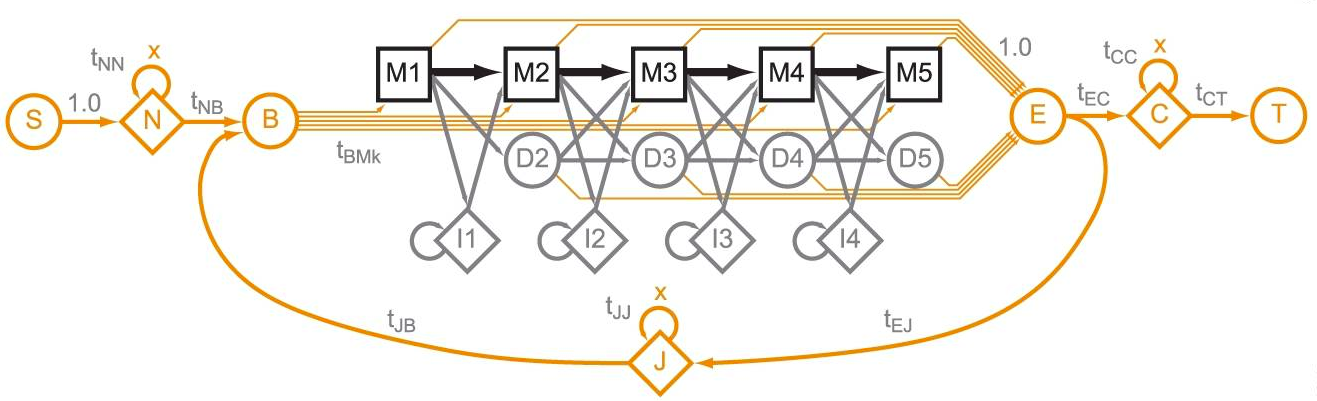
\includegraphics[width=\columnwidth]{HMM.png}
  \caption{Пример скрытой марковской модели, описывающей профиль семейства
   протеинов~\cite{MSV_Eddy}}
  \label{HMM_example}
\end{figure}
Для каждого состояния автомата заданы вероятности, возможно нулевые, которые 
определяют, символ какой аминокислоты будет выделен.
При решении задачи гомологичности рёбра переходов между состояниями помечены
весами, а не вероятностями.
Это изменение не влияет на корректность.
Используемые для описания профиля семейства СММ имеют следующую структуру.
Состояния с префиксом M содержат информацию о совпадающих аминокислотах 
семейства на определённых позициях.
Состояния с префиксом D позволяют имитировать отсутствие аминокислот у 
некоторых протеинов семейства в конкретных местах.
Состояния с префиксом I учитывают возможность произвольного количества 
вставок аминокислот.
Дополнительные состояния N, J и C моделируют негомологичные участки протеинов в 
начале, середине и конце соответственно.
Состояние S стартовое, B указывает на начало обработки гомологичного участка, E 
--- на конец этого участка, и T является завершающим состоянием.
Алгоритм проверки гомологичности принимает на вход исследуемый протеин и 
профиль семейства.
Далее выполняется алгоритм Витерби~\cite{Viterbi} для определения наиболее 
вероятных состояний в СММ с учетом наблюдаемой символьной последовательности 
исследуемого протеина.
Результатом работы является оценка гомологичности протеина и 
семейства, заданного с помощью СММ.

\subsubsection{\name{HMMer}}
\name{HMMer}~\cite{HMMer} используется для поиска в базах данных 
последовательностей гомологов исследуемых протеинов, а также для создания 
профилей семейств протеинов.
Это проект с открытым исходным кодом.
Написан на языке \name{C} с возможностью использовать \name{SIMD} инструкции 
процессора.
Применяется во многих базах данных, таких как \name{Pfam}~\cite{Pfam}.

Авторами проекта были предложены вероятностные фильтры, которые используют СММ 
из подраздела~\ref{HMM_solution} с частью удалённых состояний.
Применение фильтров позволяет ускорить обработку данных за счет уменьшения
вычислений в алгоритме Витерби.
Один из таких фильтров --- \name{MSV} (Multiple Segment 
Viterbi)~\cite{MSV_Eddy}.
Он моделирует последовательность из одной или более частей, внутри которых
аминокислоты не могут быть удалены или вставлены.
Соответственно, вероятности перехода в состояния с префиксами D и I считаются 
нулевыми (рис.~\ref{MSV_example}).
\begin{figure}[b]
  \centering
  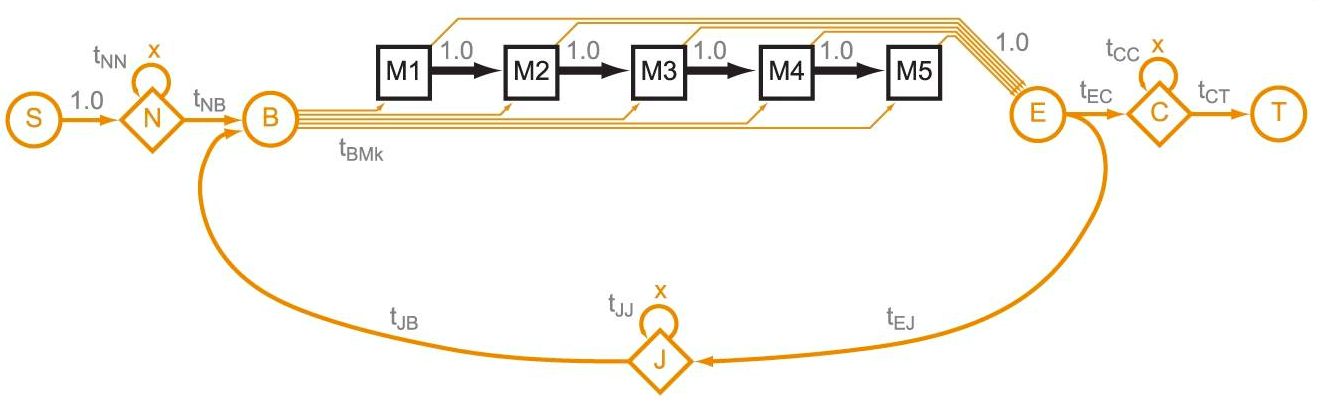
\includegraphics[width=\columnwidth]{MSV.png}
  \caption{Пример СММ фильтра MSV~\cite{MSV_Eddy}}
  \label{MSV_example}
\end{figure}

\subsubsection{\name{CUDAMPF}}
В проекте \name{CUDAMPF}~\cite{cudampf} реализованы вероятностные фильтры из 
\name{HMMer} с использованием \name{CUDA}.
Код предназначен для видеокарты \name{NVIDIA} \name{Tesla K40} архитектуры
\name{Kepler}.
Проект рассчитан на определение гомологичности одновременно для множества 
протеинов.

Авторы предлагают четыре уровня параллелизма.
Первые три основаны на логическом параллелизме по данным, так как результаты 
проверки одного протеина не зависят от другого исследуемого протеина.
Четвертый уровень использует \name{SIMD} инструкции вычислителей видеокарты.

Несмотря на то, что авторами заявлена 100\% точность, в коде фильтров
некорректно вычисляется состояние E при обработке СММ, описанной в 
подразделе~\ref{HMM_solution}.
Для этого состояния необходимо искать максимум на текущем шаге из состояний с 
префиксом M.
В исходном коде \name{CUDAMPF} переменная, хранящая максимум, не защищена от 
одновременной записи двумя или более потоками.

\subsection{Специализация GPGPU кода}
При имеющейся программе $P$ и всех её входных параметрах $inp$, можно получить 
результат выполнения $P$ на $inp$.
При наличии только части параметров $inp_1$ из $inp$, \emph{специализатор} 
должен выполнить все возможные вычисления и оптимизации кода в $P$, зависящие 
от $inp_1$, а затем сгенерировать программу $P_1$, которая будет принимать 
оставшиеся параметры $inp_2$ и выполнять последующие вычисления.
Параметры $inp_1$ называются статическими, а $inp_2$ --- динамическими.
Результат выполнения $P_1$ на $inp_2$ должен быть равен результату выполнения 
$P$ с параметрами $inp$.

Основная цель специализации GPGPU кода заключается в том, чтобы статические 
параметры были явно прописаны в коде программы.
Учитывая область применения гетерогенных систем, объем данных гораздо 
больше размера кэша данных.
Если размер ядра меньше, чем кэш кода, то специализация может увеличить 
производительность за счет того, что статические данные будут считываться из 
кэша кода, тем самым освобождая место в кэше данных.
Таким образом, уменьшается вероятность промаха кэша данных, что критически 
сказывается на скорости доступа к данным.
Например, специализация GPGPU кода алгоритма наивного поиска подстроки в строке 
дает прирост производительности в 8 раз, где статическим 
параметром была искомая подстрока~\cite{part_eval_GPU}.


\setmonofont[Mapping=tex-text]{CMU Typewriter Text}
\bibliographystyle{ugost2008ls}
\bibliography{diploma.bib}
\end{document}
